\section{$\Delta$Q display}
    Now that we have introduced the required concepts, we can put everything together to be plotted. In summary, a probe's displayed graph must contain the following functions:
    \begin{itemize}
        \item The observed $\Delta$Q at time t, with a mean and confidence bounds of previous observed $\Delta$Qs.
        \item If applicable, the calculated $\Delta$Q from the causally linked components observed in a probe, with a mean and confidence bounds of previous calculated $\Delta$Qs.
        \item Its QTA (if defined).
    \end{itemize}
    This allows for the user to observe if a $\Delta$Q has deviated from normal execution, analyse its stationarity, nonlinearity and observe its execution.

    In the photo below we can observe the multiple elements as they are displayed in real time in the oscilloscope.
    \begin{itemize}
        \item (1): The \textbf{Observed $\Delta$Q}.
        \item (2): The \textbf{Calculated $\Delta$Q}.
        \item (3): The \textbf{QTA}.
        \item Arrow, blue, below: The mean of the observed $\Delta$Qs (yellow) with the confidence bounds of the mean. Upper bound (dark green) and lower bound (light green).
        \item Arrow, red, above: The mean of the calculated $\Delta$Qs (ochre) with the confidence bounds of the mean. Upper bound (purple) and lower bound (magenta).
    \end{itemize}
     \begin{figure}[H]
        \begin{center}
            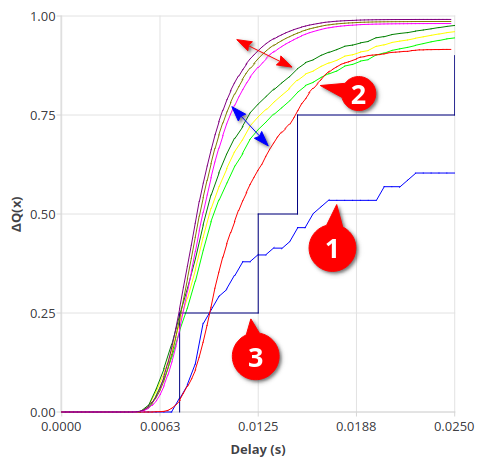
\includegraphics[scale = 0.7]{img/overload_2/qta_triggerd2.png}
        \end{center}
         \caption{$\Delta$Qs, confidence bounds, means and QTA for a probe observing the causal link of multiple components.}
    \end{figure}
        

